\documentclass{exam}
\usepackage{graphics}
\usepackage{ctex}
\begin{document}
\title{手册}
\maketitle
\newpage
\tableofcontents
\newpage


\section{平台硬件搭建}

\subsection{硬件清单}
硬件平台包含五台服务器,其中2台为GPU计算服务器,3台为CPU计算服务器。详细清单如下表:

\begin{table}[h]
\centering
\caption{硬件清单}
\begin{tabular}{ccc}
\hline\hline
设备&型号&数量\\\hline
GPU计算服务器&AMAX&2\\
CPU计算服务器&MIWIN&3\\
GPU&NVIDIA 1080&4\\
GPU&NVIDIA TITAN X&4\\
CPU&Intel Xeon E5-2698 v4&5\\
RAM&64 GB 2,133 MHz DDR4 LRDIMM&2\\
RAM&128 GB 2,133 MHz DDR4 LRDIMM&3\\
存储&1 TB HDD&4\\
\hline\hline
\end{tabular}
\end{table}

\subsection{硬件平台照片}
\begin{figure}
\centering
\includegraphics[width=0.8\hsize]{fig/d-overview.jpg}
\caption{硬件设备概览}
\end{figure}

\begin{figure}
\centering
\includegraphics[width=0.8\hsize]{fig/d-gpu.jpg}
\caption{GPU服务器机柜图}
\end{figure}

\begin{figure}
\centering
\includegraphics[width=0.8\hsize]{fig/d-cpu1.jpg}
\caption{CPU服务器图1}
\end{figure}

\begin{figure}
\centering
\includegraphics[width=0.8\hsize]{fig/d-cpu2.jpg}
\caption{CPU服务器图2}
\end{figure}

\newpage
\section{软件平台描述}
\paragraph{软件平台:}操作系统为Ubuntu Mate 16.04,使用的编程语言为64位的Python,版本为3.5.3,基于Amaconda4.4.0发行版。使用的第三方软件库包括numpy,版本为1.12.1,matplotlib,版本为2.0.2,tensorflow,版本为0.10,如图\ref{os}、\ref{py}所示。



\begin{figure}[h]
\centering
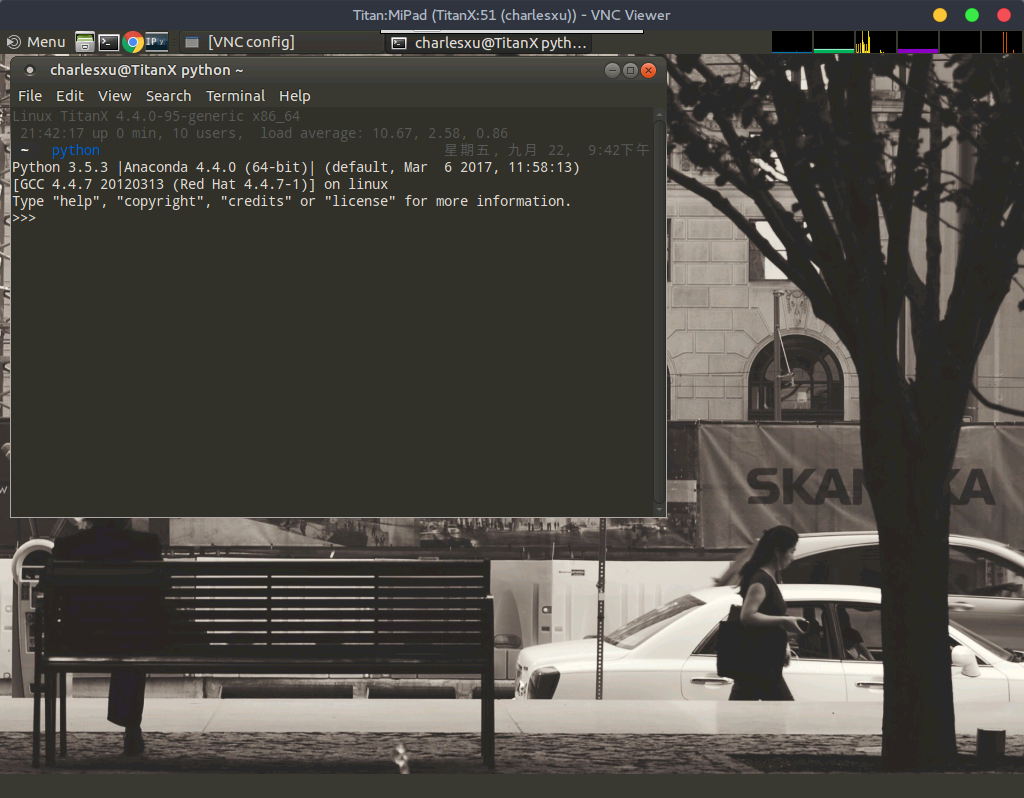
\includegraphics[width=0.8\hsize]{fig/os.png}
\caption{操作系统}
\label{os}
\end{figure}

\begin{figure}[h]
\centering
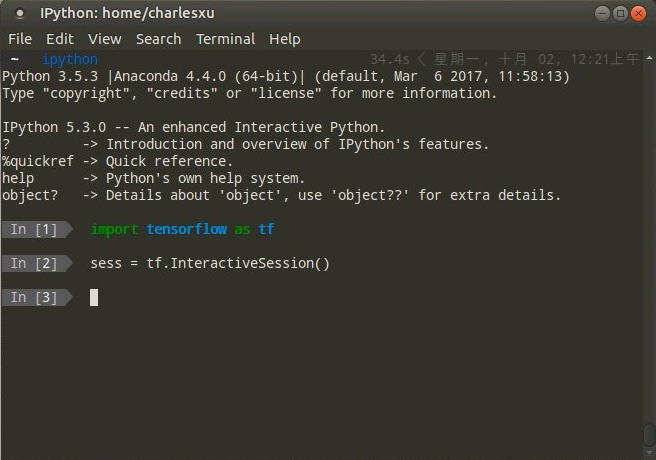
\includegraphics[width=0.8\hsize]{fig/python.jpg}
\caption{Python界面}
\label{py}
\end{figure}


\section{实验过程}

\subsection{数据准备与预处理}
\subsubsection{数据预处理}
由于本项目为单分类问题,将数据进行归一化,并将标签进行One-Hot编码。进行特征选择,筛选掉无效(即不变)特征,得到数据集,其中每条数据都是特征$\rightarrow$标签的映射对,以便之后的分析。
\subsubsection{数据可视化}
首先对数据进行可视化分析,查看数据之间的关系,分析数据的特征。如图\ref{feat},通过数据可视化,显示出在第二维和第三维特征下的不同类别数据分布图。

\begin{figure}
\centering
    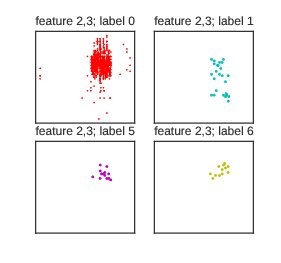
\includegraphics[width=0.4\hsize]{fig/cd/data_features.eps.png}
    \caption{数据特征可视化}
    \label{feat}
\end{figure}

\subsection{使用BP神经网络进行数据拟合}
将数据输入到神经网络中,进行初步训练,并将神经元网络的效果作为分类效果的参考标准。基于神经元网络的特点,设计如图\ref{nn}

为使神经网络训练达到最好的效果,使用“批量训练”的方法进行梯度下降优化;从数据中抽取一定量的数据作为测试数据集选择神经网络最优参数,并最终训练得到在当前数据下泛化性能最优的神经网络模型。参数选择的方法为:先采取最小网络规模,对神经网络进行训练
,并在每一轮训练后加大网络模型的广度(即每层网络中神经元数量)直到网络误差不再减小为止,增加网络的深度,继续进行搜索,直到获得最优规模的神经网络。

\begin{figure}
\centering
    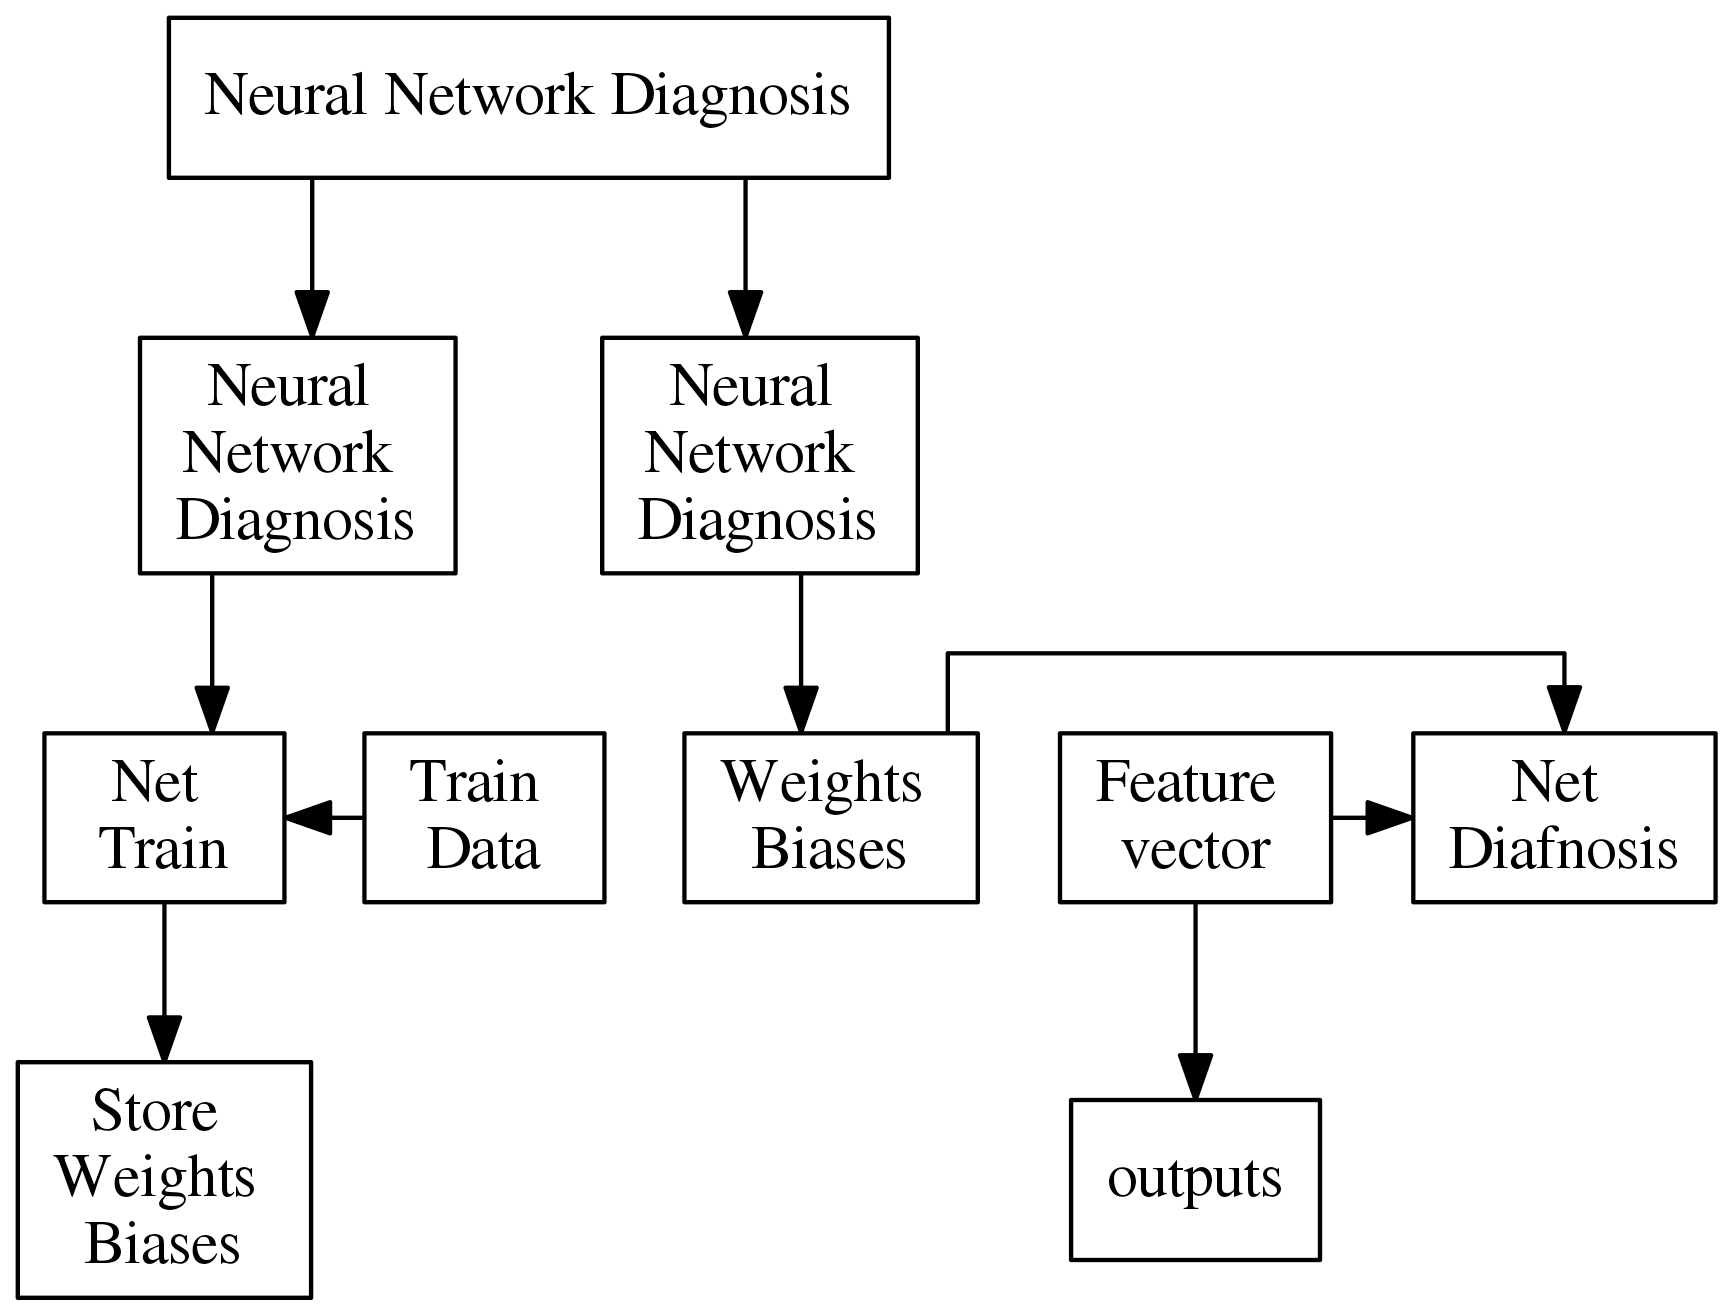
\includegraphics[width=0.8\hsize]{fig/cd/procedure.eps.png}
    \caption{神经网络故障诊断流程图}
    \label{nn}
\end{figure}

\subsection{使用自动编码器改进模型}
为了解决传统的神经网络到一定层数之后误差非降反升的问题,采取更加先进的自动编码器对数据进行降维、编码,以使神经网络的训练更加容易。

首先使用自动编码器进行数据降维,为了检验信息损失程度,将子编码还原的图像与原图像进行对比,如图\ref{ae_re}所示。使用自动编码器编码后得到编码特征如图\ref{ae_enc}所示,所编码得到的特征比图\ref{feat}的原始特征更加显著,对于分类器的训练起到促进作用。

\begin{figure}
\centering
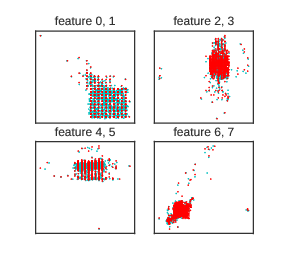
\includegraphics[width=0.4\hsize]{fig/cd/autoencoder_restore.eps.png}
\caption{自编码还原效果}
\label{ae_re}
\end{figure}

\begin{figure}
\centering
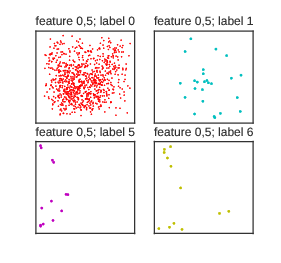
\includegraphics[width=0.4\hsize]{fig/cd/autoencoder_encoded_features.eps.png}
\caption{自编码编码后的特征图}
\label{ae_enc}
\end{figure}
\subsection{使用降噪自编码与DropOut改进自编码}
自动编码器虽然在增加网络层数的时候对训练集的拟合比神经网络要好,在训练时却更加难以训练,因为经常出现过拟合而导致模型训练失败。为了解决这个问题,加入了对自编码的两个改进,同时使用降噪自编码和DropOut对自编码容易进入过拟合的问题进行改善。实验证明,分类效果具有显著提升,训练时也不易进入过拟合。
\end{document}
